% !TEX root = ../../buch.tex
% problemstellung.tex -- Beispiel-File für die Beschreibung des Problems
%
% (c) 2020 Prof Dr Andreas Müller, Hochschule Rapperswil
%
\section{Problemstellung
\label{burgers:section:problemstellung}}
\rhead{Problemstellung}

	Das Ziel dieses Papers ist die numerische Berechnungen der Gleichung von Burgers mit ihren Schwierigkeiten aufzuzeigen.
	Die nicht lineare Eigenschaft der Gleichung erschwert die numerische L\"osung stark.
	 
	
	\subsection{Numerische Wetter Vorhersage}
	\label{burgers:sec:nwp}
	
	Die numerische L\"osung von nicht linearen partiellen Differentialgleichungen zeigten bereits in den 30er Jahren als eine grosse Herausforderung.
	Lewis Fry Richardson (1881 - 1953) war ein Britischer Mathematiker/Physiker, welcher als einer der ersten Personen versuchte das Wetter mittels numerischen Berechnungen der fundamentalen Differentialgleichungen hervorzusagen.
	F\"ur eine Hervorsage von Sechs Stunden ben\"otigte er mit seinem Team um die Sechs Wochen.
	Das Resultat war ern\"uchternd uns schlichtweg falsch.
	Es stellte sich heraus, dass Richardson einen Algorithmus verwendete welcher numerische instabil war.
	Im Verlauf des Papers werden wir sehen welcher Fehler begangen wurde.
	
	\subsection{Notation}
	
     \begin{figure}
       \centering
       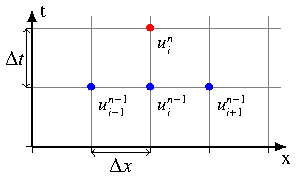
\includegraphics[height=.4\textwidth]{papers/burgers/BurgersEquation/tikz/Gitter/gitter.pdf}
       \caption{Notation Diskretisierung}
       \label{burgers:fig:Disk}
     \end{figure}
     

     Wie es bei der numerischen L\"osung von partiellen Differentialgleichungen \"ublich ist wird die Raum-Zeit Ebene  diskretisiert.
     Die gew\"ahlte Notation f\"ur die Diskretisierung kann \ref{burgers:fig:Disk} entnommen werden.
     Wobei $u_i^n$ der zu berechnende Punkt ist.
     Weiter ist $i-1$ Schritt zur\"uck im Raum und $n-1$ ein Schritt zur\"uck in der Zeit ist.
     $\Delta x$ und $\Delta t$ sind die Schrittgr\"ossen in der entsprechender Dimension, welche entgegengesetzt der Abbildung \ref{burgers:fig:Disk} nicht gleich gross sein m\"ussen.
     